\documentclass{article}
\usepackage{Self_Style}

\title{UChicago REU Notes Week 4}
\author{Zih-Yu Hsieh}
\date{\today}

\begin{document}
\maketitle
\tableofcontents

\begin{rem}
Assume everything is compactly generated, so we have a natural homeomorphism $\mathcal{U}(X\times Y,Z)\cong \mathcal{U}(X,\mathcal{T}(Y,Z))$, and $\mathcal{T}(X\wedge Y,Z)\cong \mathcal{T}(X,\mathcal{T}(Y,Z))$. Here, $\mathcal{U}$ are compactly generated spaces, $\mathcal{T}$ are based spaces.

For basic reviews of $G$-spaces, I'll type up the notes later.

Here, we also assume $V$ is a finite dimensional $\RR$-inner product space with a $G$-representation.
\end{rem}

\section{Basics of Equivariant Homotopy}


\section{Motivation of Categorical Aspect}

\textbf{Goal:} Understand to construct genuine $G$-spectra. A naive $G$-spectra is a spectra with a $G$-action (suposedly the structure maps are all $G$-equivariant + homotopy equivalence, or homeomorphism).Seems like we require extra structures on the spectra. One of the distinction seems to be: naive $G$-spectra represents $\ZZ$-graded cohomology theories, genuine $G$-spectra are used to represents cohomology theories for real representations (so it's also encoded using representations). I particular, understanding what is the equivariant infinite loop space machine (construct from $G$-space / category, forming a $G$-spectra).

\hfil

\begin{defn}
Given a category $\mathcal{V}$, $X\in\mathcal{V}$ is a $G$-object if it has a group homomorphism $G\rightarrow \Aut(X)$. 

$\mathcal{V}_G$ denotes the category of $G$-objects, with morphisms being in $\mathcal{V}$.Each $\mathcal{V}(X,Y)$ has a natural $G$-action by conjugation, where $g\in G$ acts as $f\mapsto g\circ f\circ g^{-1}$.

$G\mathcal{V} \subseteq \mathcal{V}_G$ denotes the subcategory where homsets are limited to $G$-maps (so $G\mathcal{V}(X,Y):= \mathcal{V}(X,Y)^G$, fixed points of the homsets). Another notation is $G\mathcal{V}:= (\mathcal{V}_G)^G$.
\end{defn}

\hfil

\begin{defn}
Given $X\in G\mathcal{T}$ (based $G$-space), assume inclusion of basepoint $*\rightarrow X$ is nondegenerated in the $G$-case, meaning it's a $G$-cofibration (satisfying $G$-homotopy extension property for $G$-equivariant maps, abbreviated as $G$-maps). In particular, all the homotopies in the extension property is required to be a $G$-map at all time $t$ (another way of phrasing, interval $I$ has trivial action, so action at slice $X\times t$ is equivalent to action on $X\times I$).

By chasing through the homotoopy extension diagram (by restricting all homotopies to be $G$-homotopy), then inclusion of basepoint $*\rightarrow X^H$ becomes a cofibration with respect to $G$-maps (Note: Not necessarily a $G$-cofibration, because in general $X^H$ is not closed under $G$-action). However, since all $G$-space is naturally an $H$-space (so is homotopy), then we can understand this as ``$H$-cofibration'', as $H$ acts trivially on $X^H$ :0
\end{defn}

\hfil

\begin{defn}
A $G$-map $f:X\rightarrow Y$ is a weak equivalence of $G$-spaces (or $G$-equivalence), if the fixed point maps $f^H:X^H\rightarrow Y^H$ are weak homotopy equivalences for all subgroups $H\leq G$.

Similar $G$-whiteheads theorem states if $X,Y$ are $G$-CW complexes, then $f$ is also a $G$-homotopy equivalence.
\end{defn}

\begin{defn}
    A small category $\mathcal{C}$ is a \emph{topological category}, if the set of objects $\Ob$ and set of all morphisms $\Mor$ are topological spaces, such that the following four maps are continuous:
    \begin{itemize}
        \item Identity map $i:\Ob\rightarrow\Mor$ by $i(x):=\id_x$ is a continuous map.
        \item Source map $s:\Mor\rightarrow\Ob$ by $s(f:X\rightarrow Y):= X$ is continuous.
        \item Target map $t:\Mor\rightarrow\Ob$ by $t(f:X\rightarrow Y):=Y$ is continuous.
        \item Composition $\circ:\Mor\times_{t,s}\Mor\rightarrow\Mor$ is continuous.
    \end{itemize}
    Which, the last one is collecting all pair $(X,Y)$ with morphism $f:X\rightarrow Y$ between them.
\end{defn}

In particular, $s,t$ are retracts of $i$, showing $i$ is an embedding. (check https://mathoverflow.net/questions/85717/segals-original-definition-of-a-topological-category)

There is another notion enriched over $\mathcal{T}$.

\begin{notn}
    Let $\Cat$ denotes the category of small topological categories, which $\Cat_G$ denotes the topological $G$-categories (meaning $G$ acts on both $\Ob,\Mor$ such that $i,s,t,\circ$ are all $G$-maps), an equivalent formulation is a group homomorphism $G\rightarrow \Aut_\Cat(\mathcal{C},\mathcal{C})$, by checking the definition.
\end{notn}

Part of the reason we endow this definition, is so that for subgroup $H\leq G$, the \emph{$H$-fixed category} $\mathcal{C}^H$ will make sense, namely we need the action on $\Ob,\Mor$ to be compatible.

\begin{rem}
    Given the classifying space functor $B$, it realizes any topological category $\mathcal{C}$ into $B\mathcal{C}$. 

    Question: Whatare the comparison between the two spaces?
\end{rem}

Which, for some reason it's product preserving, and it sends objects in $\Cat$ to $\mathcal{U}$, $G\Cat$ to $G\mathcal{U}$. In particular, it preserves the operad action (as preserving product also preserves the action).

\newpage

\section{$E_V$ Operads, $V$-fold Loop $G$-Spaces}

\subsection{Little Disks / Steiner Operad}

\begin{defn}
    Given $D(V)\subset V$ the open unit disk (all $v\in V$ with $\|v\|<1$), a \emph{little $V$-disk} is an affine map $d:D(V)\rightarrow D(V)$, meaning all $d(v)=r v+v_0$, where $r\in [0,1)$ and $v_0\in D(V)$ represents the radius and the center.

    Define group action $g\in G$ on collection $(g d)(v):= r v+g v_0$, which forms an evident $G$-action with restriction of action $G\rightarrow O(V)$ (the real unitary group of $V$).

    \hfil

    Define the \emph{little disk operad} by definig $\mathcal{D}_V (j):= \{(d_1,...,d_j)\ |\ d_i \text{ shares empty image intersection}\}$. Geometrically, it's all the possible arrangment of $j$ non-overlapping disks in $D(V)$. Define the evident structure map $\gamma:\mathcal{D}_V (k)\times \mathcal{D}_V (j_1)\times...\times \mathcal{D}_V (j_k)\rightarrow \mathcal{D}_V (j)$ as follow:
    \[\gamma((d'_1,...,d'_k); (d_{1,1},...,d_{1,j_1}),...,(d_{j_k,1},...,d_{j_k,j_k})) = ((d'_1\circ d_{1,1},...,d'_1\circ d_{1,j_1});...;(d'_k\circ d_{j_k,1},...,d'_k\circ d_{j_k,j_k}))\]
    Geometrically, it's as follow (for an example):
    \begin{figure}[h!]
        \centering
        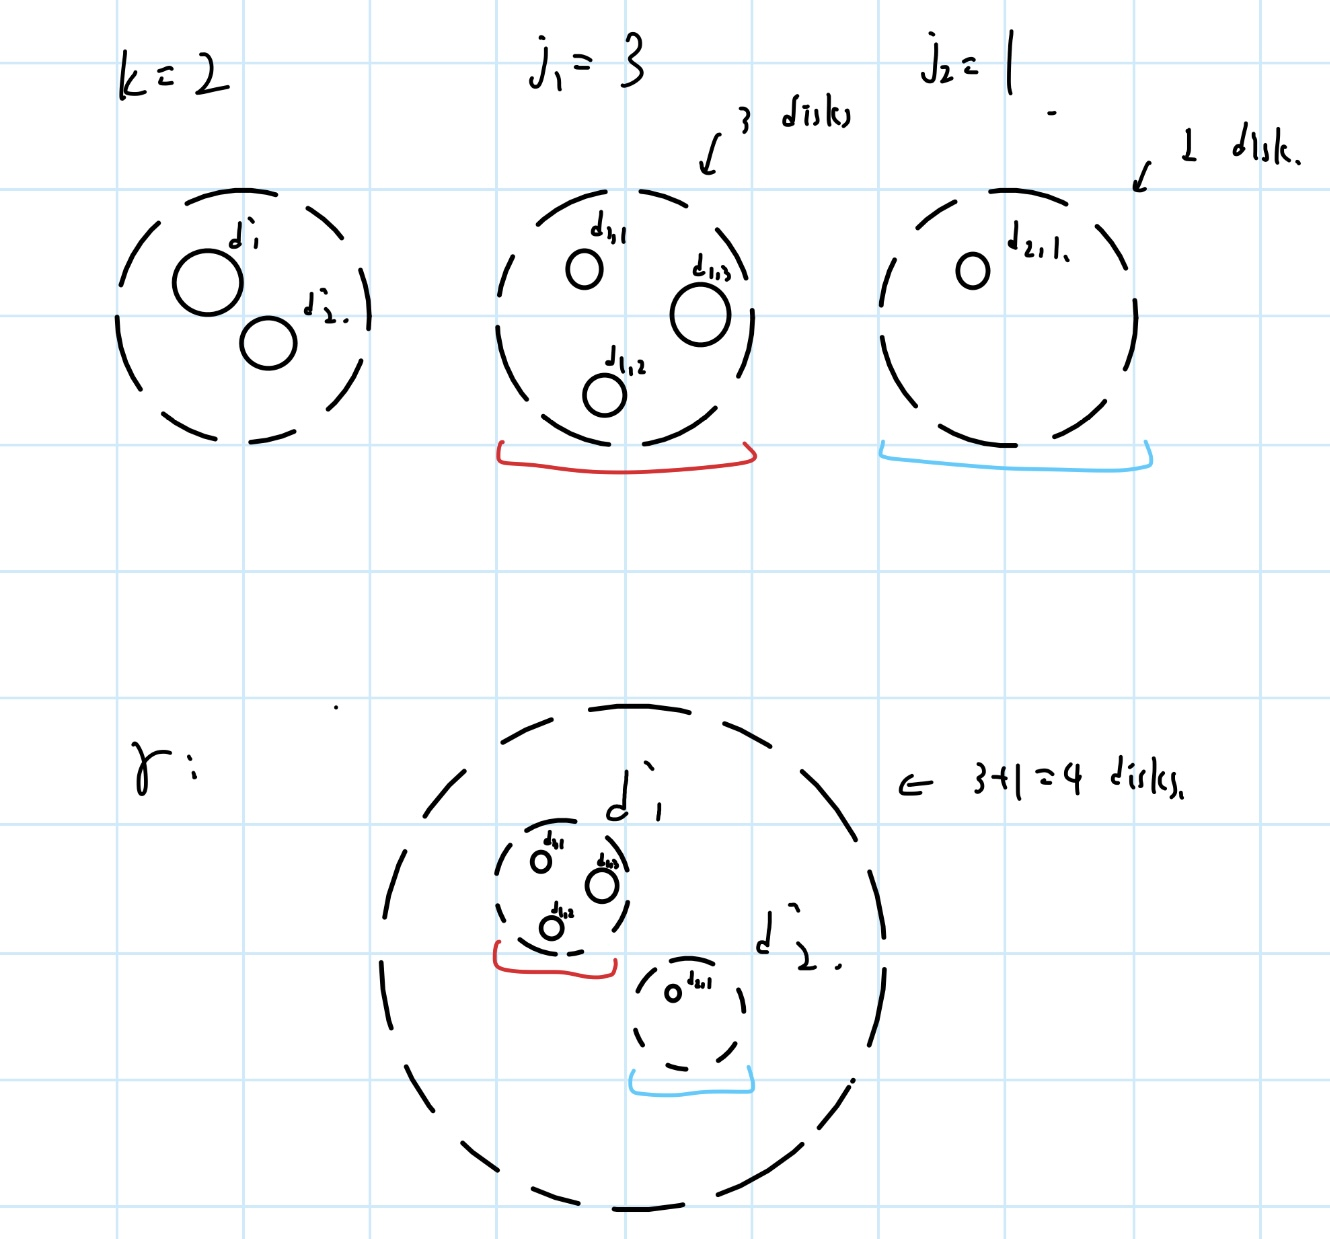
\includegraphics[width=100mm]{little disk.jpg}
    \end{figure}
\end{defn}

This is obvious a $\Sigma$-operad (as we defined it to be function composition). There is a correspondance of this definition to configuration space: Let $F(V,j)\subset V^j$ be the ordered configuration space of $j$-tuples of distinct points of $V$, with $G$ acts on $V^j$ diagonally (which restricts to an action on $F(V,j)$).

\end{document}